\chapter{Теория рассеяния}

\section{Постановка задачи рассеяния. Упругое рассеяние}

Сформулируем задачу рассеяния. Пусть имеется поток падающих (свободных) нерелятивистских частиц, каждая из которых обладает импульсом $\vp = \hbar \vec k$ (см. \autoref{fig:19_1}).

\begin{figure}[h!]
\centering
\begin{tikzpicture}[domain=-5:5]
  \draw[->] (-5, 0) -- (5, 0) node[above] {$z$};
  \draw[thick, ->] (-5, 0) -- (-4, 0) node[above] {$\vp$};
	\node [below] at (-4, 0) {падающая};
	\node [below] at (-4, -0.5) {плоская волна};
  \draw[->] (0, 0) -- (3,3);
  \draw[very thick, ->] (2.7, 2.7) -- (3,3) node [below] {$\vsp$};
  \draw[very thick, ->] (0, 0) -- (2.3,2.3) node [below] {$\vr$};
  \draw[very thick, -] (2.8, 3.3) -- (3.6,3.3) ;
  \draw[very thick, -] (3.6, 3.3) -- (3.3,3) ;
  \draw[-] (0, 0) -- (2.8,2.4);
  \draw[-] (0, 0) -- (2.4,2.8);
  \node [right] at (1, 2.2) {$d\Omega$} ;
  \node at (-2, 2) {радиус действия};
  \node at (-2, 1.5) {потенциала};
  \draw [rotate = -45] (0, 3.75) ellipse (3mm and 2 mm) ;
  \draw [dashed] (0, 0) circle (15mm);
	\draw [-, thick] (0, 0) circle (2mm);
	\node [below] at (0, -0.1) {рассеивающий};
	\node [below] at (0, -0.6) {центр};
  \node [below] at (4, 2.5) {рассеянная};
	\node [below] at (4, 2) {волна};
  \draw [->] (0, 0) -- (-1.06, 1.06) node [left] {$a$}; 
  \draw [thick,->] (1, 0) arc (0:45:10mm);
	\draw [rotate=-45, ->, thick] (2.5, 2.2) arc (0:-270:3mm);
  \draw [fill] (3.1, 0) circle (0.5mm);
	\node [above] at (3.6, 0) {$\phi$};
  \node [right] at (0.6, 0.3) {$\theta$};
  \draw [blue, dashed] (-3, 0) .. controls (0, 0) .. (3, 3);
\end{tikzpicture}
\caption{Постановка задачи рассеяния.} \label{fig:19_1}
\end{figure}

Выберем начало координат в той области, где отличен от нуля рассеивающий потенциал. Предположим, что эта область ограничена радиусом $a$, так что
$$
U(\vr) \equiv 0, \text{ если } r > a
$$

Подчеркнем, что внутри сферы радиуса $a$ потенциал $U(\vr)$ имеет произвольную форму. Требуется найти зависимость потока рассеянных частиц от направления рассеяния.

Формально задача описывается уравнением Шрёдингера
\begin{equation}
\label{eq:19_1_1}
\op{H} \psi(\vr) = E \psi(\vr),
\end{equation}
с гамильтонианом $\op{H} = \dfrac{\op{\vp}^2}{2m} + U(\vr)$. В случае, когда $E < 0$, речь идет о поиске связанных состояний. Напомним, что волновая функция частицы, находящейся в связанном состоянии, удовлетворяет граничному условию:
$$
\psi(\vr) \to 0 \text{ при } r \to \infty
$$

В случае задачи рассеяния энергия фиксирована (задана) и положительна:
$$
E = \frac{\hbar^2 k^2}{2m} > 0,
$$
т.е. волновая функция $\psi(\vr)$, описывающая процесс рассеяния частицы на потенциале $U(\vr)$, принадлежит непрерывному спектру гамильтониана \eqref{eq:19_1_1}. Для состояний непрерывного спектра $\psi(\vr)$ необходимо конкретизировать граничные условия на бесконечности (асимптотику).

Будем считать рассеяние упругим, т.к. энергия до и после рассеяния одна и та же: $\dfrac{p^2}{2m} = \dfrac{p'^2}{2m}$, но вектор импульса $\vp$ поворачивается на угол $\theta$ (см. \autoref{fig:19_1}), т.е. 
$$
\vp \neq \vsp,~~~\abs{\vp} = \abs{\vsp} = \hbar k
$$

На больших расстояниях, где потенциалом $U(\vr)$ можно пренебречь, волновая функция частицы представляет собой суперпозицию падающей плоской волны и рассеянной волны. Рассеянная волна на бесконечности является расходящейся сферической волной, т.к. любая ограниченная область по отношению к бесконечности может быть принята за точку. Следовательно, в асимптотике $r \to \infty$ волновая функция частицы в задаче рассеяния должна иметь вид:
$$
\left . \psi(\vr) \right|_{r \to \infty} \approx e^{i \vec{k} \vr} + f(\theta, \phi) \frac{e^{ikr}}{r}
$$

Углы $\theta$ и $\phi$ --- это полярный и азимутальный углы, которыми определяется направление радиус-вектора $\vr$ (см. \autoref{fig:19_1}). Функцию $f(\theta, \phi)$ называют амплитудой рассеяния. Для произвольного потенциала $U(\vr)$ амплитуда зависит от $\theta$ и $\phi$, но если $U(\vr)$ --- центрально-симметричное поле, то амплитуда от $\phi$ не зависит. Задача рассеяния с аксиальной симметрией имеет асимптотику:
\begin{equation}
\label{eq:19_1_2}
\left . \psi(\vr) \right|_{r \to \infty} \approx e^{i \vec{k}\vr} + f(\theta) \frac{e^{ikr}}{r}
\end{equation}

Волновые функции, имеющие асимптотический вид \eqref{eq:19_1_2}, мы будем называть волновыми функциями рассеяния, а задачу их отыскания --- прямой задачей рассеяния.

\section{Амплитуда и сечение рассеяния}

Амплитуда $f(\theta, \phi)$ не является непосредственно измеряемой величиной. В экспериментах принято изменять сечение рассеяния. Регистрация рассеянных частиц под углами $\theta$ и $\phi$ осуществляется детектором, охватывающим телесный угол $d\Omega$ (см. \autoref{fig:19_1}). Скорость счета детектора $\dfrac{dN}{dt}$ --- это число частиц, попадающих в детектор в единицу времени.

\begin{defn}
Плотность потока падающих частиц $\vec{j}_{\text{пад}}$ --- число частиц, проходящих в единицу времени через единичную площадку, перпендикулярную к пучку.
\end{defn}

\begin{defn}
Отношение скорости счета детектора к плотности потока падающих частиц называется эффективным сечением (или просто сечением) рассеяния:
\begin{equation}
\label{eq:19_2_1}
d \sigma = \frac{1}{j_{\text{пад}}}\frac{dN}{dt},
\end{equation}
где $\brs{d\sigma} =\brs{\dfrac{1}{\text{сек}}:\dfrac{1}{\text{сек} \cdot \text{см}^2}} =[\text{см}^2]$.
\end{defn}

С другой стороны, скорость счета детектора дается выражением:
$$
\D{N}{t} = j_{\text{рас}}r^2 d\Omega,
$$
где $j_{\text{рас}}$ --- плотность потока рассеянных частиц. Тогда сечение рассеяния \eqref{eq:19_2_1} можно записать в виде:
\begin{equation}
\label{eq:19_2_2}
d\sigma = \frac{j_{\text{рас}}}{j_{\text{пад}}}r^2 d\Omega
\end{equation}

Определение \eqref{eq:19_2_2} применимо не только в классической, но и в квантовой механике. Действительно, классическая плотность потока частиц в пучке пропорциональна плотности потока вероятности одной частицы в квантовой механике:
$$
\vec{j} = \frac{-i\hbar}{2m}\brc{\psi^* \nabla \psi - \psi \nabla \psi^*}~~~\text{   (см. \S 1 главы \rom{5})}
$$

Для падающей волны с единичной амплитудой $e^{ikz}$ плотность потока вероятности $j_{\text{пад}} = v$ (см. \S 1 главы \rom{5}) направлена по оси $z$, а в расходящейся сферической волне с плотностью вероятности $\rho_{\text{рас}} = \dfrac{\abs{f(\theta)}^2}{r^2}$ плотность потока вероятности $j_{\text{рас}} = \rho_{\text{рас}} v = v \dfrac{\abs{f(\theta)}^2}{r^2}$ направлена по радиусу. Поэтому дифференциальное сечение рассеяния равно
\begin{equation}
\label{eq:19_2_3}
\D{\sigma}{\Omega} = \abs{f(\theta)}^2
\end{equation}

Таким образом, решение задачи упругого рассеяния сводится в нахождению амплитуды рассеяния $f(\theta)$.

\section{Функция Грина задачи рассеяния. Интегральное уравнение задачи рассеяния}

Дифференциальное уравнение Шрёдингера для задачи рассеяния выглядит следующим образом:
$$
\brc{-\frac{\hbar^2}{2m} \Delta + U(\vr)}\psi(\vr) = \frac{\hbar^2 k^2}{2m} \psi(\vr)
$$

Домножение обеих частей уравнения на $\dfrac{2m}{\hbar^2}$ и перегруппировка слагаемых дает:
$$
(\Delta + k^2) \psi(\vr) = \frac{2m}{\hbar^2}U(\vr)\psi(\vr)
$$

Ищем решение этого уравнение в виде суммы общего решения однородного уравнения
$$
(\Delta + k^2) \psi_0(\vr) = 0
$$
и частного решения неоднородного уравнения
$$
(\Delta + k^2) \psi_1(\vr) = \frac{2m}{\hbar^2}U(\vr)\psi(\vr),
$$
т.е. $\psi(\vr)=\psi_0(\vr) + \psi_1(\vr)$.

Для нахождения частного решения воспользуемся функцией Грина $G(\vr - \vsr)$, которая по определению представляет собой решение следующего уравнения:
\begin{equation}
\label{eq:19_3_1}
(\Delta_{\vr} + k^2)G(\vr - \vsr) \equiv \delta(\vr - \vsr),
\end{equation}
где $\vsr$ характеризует точку источника, а $\vr$ --- точку наблюдения. Легко видеть, что
$$
\psi_1(\vr) = \int G(\vr - \vsr) \frac{2m U(\vsr)}{\hbar^2} \psi(\vsr) d\vsr
$$

В самом деле, действуя оператором $(\Delta_{\vr} + k^2)$ на обе части последнего соотношения, получаем:
$$
(\Delta_{\vr} + k^2) \psi_1(\vr) = \int \delta(\vr - \vsr) \frac{2m U(\vsr)}{\hbar^2} \psi(\vsr) d\vsr = \frac{2m U(\vr)}{\hbar^2} \psi(\vr)
$$

Найдем явное выражение для функции Грина. В теории поля уже находили функцию Грина волнового уравнения \eqref{eq:19_3_1} с правой частью $-4\pi \delta(\vr - \vsr)$. Поэтому функцией Грина, удовлетворяющей асимптотике \eqref{eq:19_1_2}, будет
$$
G(\vr - \vsr) = - \frac{e^{ik\abs{\vr - \vsr}}}{4\pi\abs{\vr - \vsr}}
$$

Общее решение уравнение Шрёдингера принимает вид
$$
\psi(\vr) = \psi_0(\vr) - \frac{1}{4 \pi}\frac{2m}{\hbar^2}\int \frac{e^{ik\abs{\vr - \vsr}}}{\abs{\vr - \vsr}} U(\vsr)\psi(\vsr)d\vsr
$$

Это решение является формальным. В самом деле, под знаком интеграла в правой части стоит та же неизвестная функция $\psi(\vr)$, что и в левой части. Поэтому правильнее было бы сказать, что мы выполнили переход от дифференциального уравнения Шрёдингера к эквивалентному интегральному уравнению.

Заметим, что подынтегральное выражение в правой части отлично от нуля только в области, где $r' < a$. Следовательно,
$$r' < a \ll r \text{ при } r \to \infty,$$
т.е. при переходе к асимптотике $r \to \infty$ возникает малый параметр $\dfrac{r'}{r} \ll 1$. Разложение по этому малому параметру дает
$$
\abs{\vr - \vsr} \approx r - \vsr \cdot \vec{n}, \text{ где } \vec{n} = \frac{\vr}{r} \text{   (см. \autoref{fig:19_1})}
$$
и
$$
\frac{e^{ik\abs{\vr - \vsr}}}{\abs{\vr - \vsr}} \approx \frac{e^{ikr - ik\vsr \vec{n}}}{r}
$$

Итак, волновая функция $\psi(\vr)$ в асимптотике принимает вид
$$
\left. \psi(\vr) \right|_{r \to \infty} = \psi_0(\vr) - \frac{e^{ikr}}{r}\frac{m}{2\pi\hbar^2}\int e^{- ik\vec{n}\vsr} U(\vsr)\psi(\vsr)d\vsr
$$

Ранее мы предположили, что волновая функция должна иметь следующую асимптотику:
$$
\left. \psi(\vr) \right|_{r \to \infty} \approx e^{i\vec{k}\vr} + f(\theta, \phi)\frac{e^{ikr}}{r}
$$

Легко видеть, что, взяв в качестве решения $\psi_0(\vr)$ однородного уравнения плоскую волну
$$\psi_0(\vr) = e^{i\vec{k}\vr},$$
мы получаем точно то, что и ожидали. При этом амплитуда рассеяния определяется следующей формулой:
$$
f(\theta, \phi) =  - \frac{m}{2\pi\hbar^2}\int e^{- ik\vec{n}\vsr} U(\vsr)\psi(\vsr)d\vsr
$$

Таким образом, мы осуществили переход от исходного дифференциального уравнение Шрёдингера к интегральному уравнению
\begin{equation}
\label{eq:19_3_2}
\boxed{\psi(\vr) = e^{i\vec{k}\vr} - \frac{m}{2\pi\hbar^2}\int \frac{e^{ik\abs{\vr - \vsr}}}{\abs{\vr - \vsr}} U(\vsr)\psi(\vsr)d\vsr}
\end{equation}

В асимптотике $r \to \infty$ решение этого уравнения имеет требуемый вид. Уравнение \eqref{eq:19_3_2} называют интегральным уравнением задачи рассеяния.

\section{Приближение Борна. Критерии применимости борновского приближения}

Если потенциал $U(\vr)$ является малым возмущением, то можно искать волновую функцию как разложение в ряд по степеням малого параметра $U$:
\begin{equation}
\label{eq:19_4_1}
\psi = \psi^\zr + \psi^\one + \dots + \psi^{(n)} + \dots
\end{equation}

При использовании $n$ членов разложения помимо $\psi^\zr$ говорят об $n$-ом борновском приближении, а при $n = 1$ говорят о первом борновском приближении (или просто борновском приближении). Из \eqref{eq:19_3_2} следует, что $\psi^\zr = e^{i \vec{k} \vr}$ и
\begin{equation}
\label{eq:19_4_2}
\psi^\one(\vr) = -\frac{m}{2\pi \hbar^2} \int \frac{e^{ik \abs{\vr - \vsr}}}{\abs{\vr - \vsr}} U(\vsr) e^{i \vec{k} \vsr} d\vsr
\end{equation}

Тогда для амплитуды рассеяния в борновском приближении получаем
$$
f(\theta, \phi) \approx  -\frac{m}{2\pi \hbar^2} \int e^{-i(\vec{k}'-\vec{k})\vsr} U(\vsr) d\vsr
$$

\begin{figure}[h!]
\centering
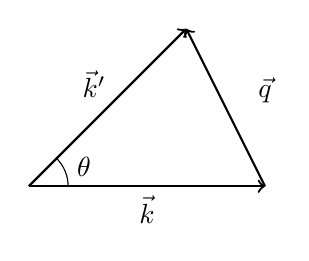
\begin{tikzpicture}[domain=-5:5]
  \draw[->, thick] (0, 0) -- (3, 0);
  \draw[->, thick] (0, 0) -- (2, 2);
  \draw[->, thick] (3, 0) -- (2, 2);  
  \node[below] at (1.5, 0) {$\vec k$};
  \node[above] at (0.7, 0) {$\theta$};
  \node[left] at (1.1, 1.3) {$\vec{k}'$};
  \node[below] at (3, 1.5) {$\vec q$};
  \draw[-] (0.5, 0) arc (0:45:5mm);  
\end{tikzpicture}
\caption{} \label{fig:19_2}
\end{figure}

Здесь $\vec{k}' = k \vec{n}$ --- волновой вектор рассеянной частицы. Вводя вектор $\vec{q} = \vec{k}'- \vec{k}$ (см. \autoref{fig:19_2}) --- вектор переданного частице рассеивающим центром импульса (в единицах $\hbar$), запишем последнее равенство в виде:
\begin{equation}
\label{eq:19_4_3}
f(\theta, \phi) \approx  -\frac{m}{2\pi \hbar^2} \int e^{-i \vec{q}\vsr} U(\vsr) d\vsr,
\end{equation}
где $q = 2k \sin \dfrac{\theta}{2}$. Если $U$ --- сферически симметричная функция, $U(\vsr) = U(r')$, то из \eqref{eq:19_4_3}, проводя интегрирование по углам, окончательно получим:
\begin{equation}
\label{eq:19_4_4}
f(\theta) \approx -\frac{2m}{\hbar^2} \int_0^\infty \frac{\sin qr}{qr}U(r)r^2 dr
\end{equation}

Выясним теперь условия, при которых формула \eqref{eq:19_4_4} применима. Критерий применимости борновского приближения выглядит как
\begin{equation}
\label{eq:19_4_5}
\abs{\psi^\one} \ll \abs{\psi^\zr} = 1
\end{equation}

Вычисляя в \eqref{eq:19_4_2} функцию $\psi^\one(\vr)$ в наиболее опасной точке $r = 0$ в смысле нарушения неравенства \eqref{eq:19_4_5}, получаем:
$$
\frac{m}{2 \pi \hbar^2} \left| \int \frac{e^{ikr'}}{r'} U(\vsr) e^{i\vec{k} \vsr}d\vsr\right | \ll 1
$$
или для сферически симметричного потенциала $U(r')$
\begin{equation}
\label{eq:19_4_6}
\boxed{\frac{m}{\hbar^2 k} \left| \int_0^a (1 - e^{2ikr'}) U(r') dr'\right | \ll 1}
\end{equation}

Далее возможны два случая.

\begin{enumerate}
\item Медленные частицы, для которых $ka \ll 1$. В \eqref{eq:19_4_6} $1-e^{2ik r'} \approx -2ikr'$ и критерий применимости имеет вид:
$$
\frac{m}{\hbar^2} \underbrace{\left| \int_0^a r' U(r') dr' \right|}_{\sim a^2 U_0} \sim \frac{m U_0 a^2}{\hbar^2} \ll 1 \text{ или } \boxed{U_0 \ll \frac{\hbar^2}{ma^2}},
$$
где $U_0$ --- характерный масштаб потенциальной энергии.

\item Быстрые частицы, для которых $ka \gg 1$. В этом случае под знаком интеграла \eqref{eq:19_4_6} присутствует быстро осциллирующая экспонента, которая зануляет часть интеграла, и критерий применимости обретает форму записи:
$$
\frac{m}{\hbar^2 k} \underbrace{\left| \int_0^a U(r') dr'\right |}_{\sim a U_0} \sim \frac{m U_0 a}{\hbar^2 k} = \frac{m U_0 a^2}{\hbar^2 (ka)} \ll 1 \text{ или } \boxed{U_0 \ll \frac{\hbar^2}{ma^2} ka}
$$
\end{enumerate}

Т.к. $ka \gg 1$, то это условие оказывается более слабым ограничением на величину взаимодействия $U_0$, чем условие для медленных частиц.
